\begin{frame}
\frametitle{EigensProvider()}
\framesubtitle{Ordinare correttamente gli autovalori non \`e facile}
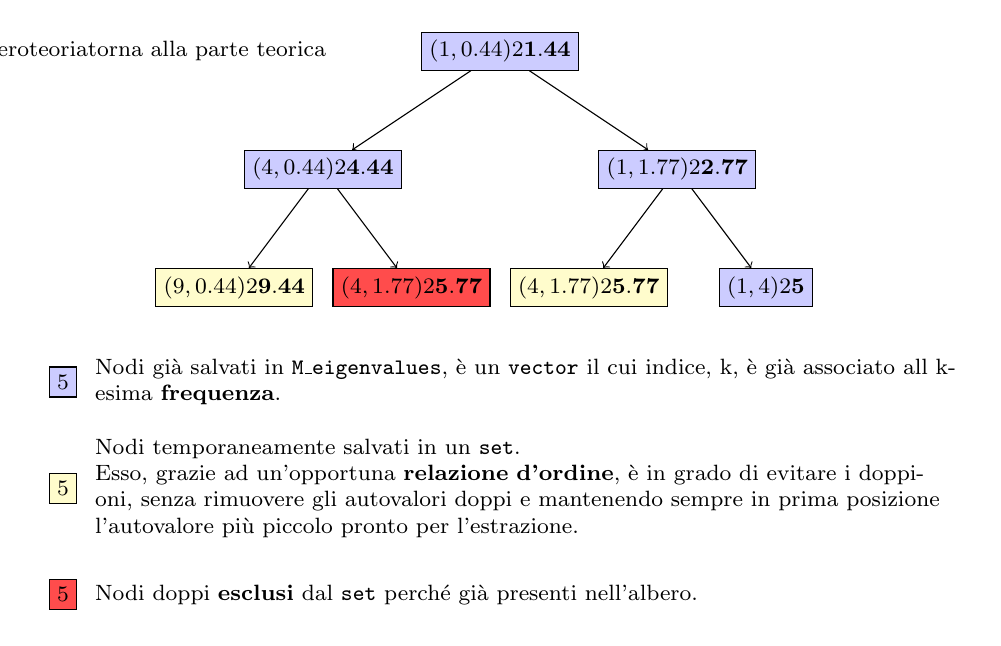
\begin{tikzpicture}
[scale=1.5]
\footnotesize
\tikzstyle{eig}=[rectangle, draw, fill=blue!20];
\tikzstyle{temp}=[rectangle,draw,fill=yellow!20];
\tikzstyle{rip}=[rectangle,draw,fill=red!70];
\def\yo{4.8}:
\def\dy{-1};
\def\c{1.5};
\def\spazio{2};
\useasboundingbox (-4,0) rectangle (4,5);
\hypertarget<1-1>{albero}{};
\node<1-> (goback) at (-3,\yo) {\hyperlink{alberoteoria}{\beamerreturnbutton{torna alla parte teorica}}};
\node<1->[eig] (v1) at (0,\yo)  {$(1,0.44)\psp{\spazio}\mathbf{1.44}$};
\node<2-4>[temp] (v2) at (-\c,\yo+\dy)  {$(4,0.44)\psp{\spazio}\mathbf{4.44}$};
\node<2-2>[temp] (v3) at (+\c,\yo+\dy)   {$(1,1.77)\psp{\spazio}\mathbf{2.77}$};
\draw<2->[->] (v1) -- (v2);
\draw<2->[->] (v1) -- (v3);
\node<3->[eig] (v3) at (+\c,\yo+\dy)   {$(1,1.77)\psp{\spazio}\mathbf{2.77}$};
\node<4->[temp] (v4) at (\c - \c/2,\yo+2*\dy) {$(4,1.77)\psp{\spazio}\mathbf{5.77}$};
\node<4-8>[temp] (v5) at (\c + \c/2,\yo+2*\dy) {$(1,4)\psp{\spazio}\mathbf{5}$};
\draw<4->[->] (v3) -- (v4);
\draw<4-8>[->] (v3) -- (v5);
\node<5->[eig] (v2) at (-\c,\yo+\dy) {$(4,0.44)\psp{\spazio}\mathbf{4.44}$};
\node<6->[temp] (v6) at (-\c-\c/2,\yo+2*\dy) {$(9,0.44)\psp{\spazio}\mathbf{9.44}$};
\node<6-6>[temp] (v7) at (-\c+\c/2,\yo+2*\dy) {$(4,1.77)\psp{\spazio}\mathbf{5.77}$};
\draw<6->[->] (v2) -- (v6);
\draw<6->[->] (v2) -- (v7);
\node<7->[rip] (v7) at (-\c+\c/2,\yo+2*\dy) {$(4,1.77)\psp{\spazio}\mathbf{5.77}$};
\node<8->[eig] (v5) at (\c + \c/2,\yo+2*\dy) {$(1,4)\psp{\spazio}\mathbf{5}$};

\def\s{-0.5};
\def\sp{0.3};
\node<1->[eig] (legeig) at (-4+\sp,\s+\yo+2.3*\dy) {$\psp{5}$};
\node<1->[right,text width=11.5cm] (texteig) at (-3.5,\s+\yo+2.3*\dy) {Nodi gi\`a salvati in \texttt{M\_eigenvalues}, 
\`e un \texttt{vector} il cui indice, k, \`e gi\`a associato all k-esima \textbf{frequenza}.};
\node<2->[temp] (legtmp) at (-4+\sp,\s+\yo+3.2*\dy) {$\psp{5}$};
\node<2->[right,text width=11.5cm] (texteig) at (-3.5,\s+\yo+3.2*\dy) {Nodi temporaneamente salvati in un \texttt{set}.\\ Esso, grazie ad un'%
opportuna \textbf{relazione d'ordine}, \`e in grado di evitare i doppioni, senza rimuovere gli autovalori doppi e mantenendo 
sempre in prima posizione l'autovalore pi\`u piccolo pronto per l'estrazione.};
\node<7->[rip] (legrip) at (-4+\sp,\s+\yo+4.1*\dy) {$\psp{5}$};
\node<7->[right,text width=11.5cm] (texteig) at (-3.5,\s+\yo+4.1*\dy) {Nodi doppi \textbf{esclusi} dal \texttt{set} perch\'e gi\`a presenti nell'albero.};
\end{tikzpicture}
\end{frame}